\documentclass{article}
\usepackage{arxiv}
\usepackage[utf8]{inputenc}
\usepackage[T1]{fontenc}
\usepackage{hyperref}
\usepackage{url}
\usepackage{booktabs}
\usepackage{amsfonts}
\usepackage{amsmath,amssymb}
\usepackage{microtype}
\usepackage{graphicx}
\usepackage{natbib}
\usepackage{doi}
\usepackage{cleveref}
\usepackage{xcolor}
\usepackage{enumitem}
\setlist{nosep,leftmargin=*}
\title{Addressable Editing for Reliable OCR Post-Correction: Interfaces, Tails, and Protocol Compliance}
\author{Author names and affiliations to be supplied}
\date{}
\renewcommand{\shorttitle}{Addressable Editing for OCR Post-Correction}
\hypersetup{pdftitle={Addressable Editing for Reliable OCR Post-Correction},pdfauthor={Author information to be supplied},pdfkeywords={OCR post-correction, LLM agents, editing interfaces, HIPE-OCRepair}}
\newcommand{\cmer}{\mathrm{cMER}}
\newcommand{\pfr}{\textsc{LocalPatch}}
\newcommand{\fr}{\textsc{FindReplace}}
\newcommand{\rewrite}{\textsc{Rewrite}}
\newcommand{\mthree}{\textsc{M3}}
\newcommand{\vfour}{\textsc{V4}}
\begin{document}
\maketitle

\begin{abstract}
Large language models can improve noisy historical OCR, but a correction that fixes a few characters may also silently rewrite or corrupt an entire document. We study whether the editing interface exposed to an agent changes this risk. We implement a block-addressable document intermediate representation (IR), content-addressable snapshots, atomic edit application, and auditable session tapes with deterministic replay. On 33 matched document tasks from the German DTA19 subset of HIPE-OCRepair-Bench, we compare eight one-shot interfaces under controlled prompts and three model configurations. With DeepSeek V4 Flash, local block-scoped find-and-replace has median cMER 0.0084, P90 0.0199, and maximum 0.0295, whereas unrestricted rewriting reaches maximum 0.9648. The same tail separation appears with DeepSeek V4.1 Flash (local patch P90 0.0187; maximum 0.0284). However, MiniMax M3 frequently fails to follow the text-tool protocol: six tool interfaces complete only 1--15 of 33 tasks, making their apparent quality indistinguishable from the no-edit anchor. We also identify a presentation confound: adding stable-looking numeric keys to a global find-and-replace view reduces the V4 correction rate by 10.3 percentage points, while the paired bootstrap interval for edit-span reduction includes zero. These results support addressable editing as a useful reliability mechanism under protocol-compliant models, and show that interface claims must report tail risk, protocol compliance, and model-interface interactions together.
\end{abstract}
\keywords{OCR post-correction \and LLM agents \and editing interfaces \and reproducibility}

\section{Introduction}
Historical collections contain systematic OCR errors, and post-correction is increasingly evaluated with large language models. The HIPE-OCRepair benchmark makes this setting reproducible and emphasizes character-level Match Error Rate (cMER), a continuous metric that exposes both improvements and severe over-correction \citep{ehrmann2026hipe}. The metric is particularly useful for agents: two systems can have similar typical scores while one has rare, catastrophic failures.

A second issue is the interface between an agent and the document. A chat model that emits a complete replacement text has a large destructive action surface. An agent that emits a verified replacement scoped to a stable block has a smaller surface, but may spend more effort locating edits or complying with a tool grammar. Prior work has shown that interfaces designed for language-model users can change software-engineering outcomes \citep{yang2024sweagent}; executable editing and audit trails have also been studied for human-facing document workflows \citep{laban2023inksync}. The effect of such choices on OCR post-correction, including the rare failures that dominate trust, has not been systematically isolated.

We make four contributions.
\begin{itemize}
  \item We introduce a reproducible block-addressable editing harness for OCR post-correction. The harness lowers agent edits through a typed addressing interface, applies IR operations atomically, stores content-addressable snapshots, and records replayable session tapes.
  \item We conduct a controlled eight-arm interface ablation on matched DTA19 German documents, separating global replacement, block-scoped replacement, attention instructions, stable identifiers, unstable positional identifiers, and full rewriting.
  \item We show that local addressability mainly separates the tail of the cMER distribution. On two DeepSeek configurations, local patching has an order-of-magnitude smaller worst case than full rewriting while central tendencies remain close.
  \item We expose a protocol and presentation confound. MiniMax M3 often does not complete the one-shot tool grammar, and adding numeric keys alone changes V4 behavior. Interface comparisons therefore require compliance and view presentation as measured factors.
\end{itemize}

Our claims are deliberately conditional. We do not claim that local editing is universally better, nor that numeric keys alone cause conservatism across models. The experiments instead provide a measurement framework and a set of falsifiable observations about reliability.

\section{Background and Related Work}
\paragraph{OCR post-correction.} HIPE-OCRepair evaluates noisy historical transcripts with cMER, wMER, and preference-oriented measures, and reports over-correction as a recurring challenge \citep{ehrmann2026hipe}. We use its released scorer and the matched DTA19 subset. Our document-level aggregation is a controlled research setting and should not be interpreted as a leaderboard score.

\paragraph{Interfaces for language-model agents.} SWE-agent frames the interface used by an LM as an agent-computer interface and shows that search, viewing, and editing primitives affect software-engineering performance \citep{yang2024sweagent}. InkSync uses executable suggestions and traces to make text editing verifiable \citep{laban2023inksync}. Recent work on structured code-edit formats likewise argues that the output representation can be as important as model capacity \citep{cheng2026diff}. We transfer this question to OCR post-correction, where the output must remain faithful to an imperfect input and rare corruption is costly.

\paragraph{Document reliability.} DELEGATE-52 reports sparse but severe document corruption over long delegated workflows \citep{laban2026delegate}. Our task is shorter and has a gold transcription, but it shares the reliability objective: measure what the system damages, not only what it fixes. Work comparing restricted tool surfaces also finds that pass rates can remain tied while cost and failure behavior change \citep{yang2026executecode}; this motivates reporting cMER tails and protocol compliance together.

\section{Addressable Editing Harness}
\subsection{Document IR and addressing}
The input transcript is partitioned into ordered blocks. A snapshot is a tuple
\[
 S=(k_1,x_1),\ldots,(k_n,x_n),
\]
where each block has an immutable key $k_i$ and content $x_i$. A tool call is parsed into a typed operation, for example
\texttt{find\_replace(path, key, old, new)}.
The parser checks the path, key, and uniqueness of \texttt{old} in the addressed block. A valid call lowers to IR operations such as \texttt{SetContent} and \texttt{Remove}. The operation list is applied as a pure function: if any operation fails, the complete list is rejected and the input snapshot remains unchanged.

The global interface uses the same replacement semantics but checks uniqueness over the complete path. The local interface checks only the addressed block. The unstable condition uses positional line identifiers and re-partitions the document after each edit; the stable condition preserves keys across edits. In all conditions, keys are view metadata and are removed before scoring.

\subsection{Snapshots, tapes, and replay}
Each session has a content-addressable store. A block blob is identified by a hash of its normalized content and attributes, while a snapshot manifest records the ordered keys and blob references. Saves use temporary files and atomic replacement. The session tape stores prompts, completions, parsed calls, tool results, status, and the final output. Replay re-runs parsing and deterministic folding from the tape without calling the model API. This separates model stochasticity from post-processing changes and makes the reported artifacts auditable.

\subsection{One-shot agent loop}
Every cell uses one document per session and a one-shot instruction. The model receives the current view and either emits a complete rewritten transcript or emits one call per line followed by \texttt{done()}. Parse errors are returned to the model in the ordinary loop; a cell that exhausts its budget is retained and scored with its extracted output. This choice measures both correction quality and the model's ability to use the interface contract.

\section{Experimental Design}
\subsection{Data and tasks}
We use the matched DTA19 German dev subset distributed with HIPE-OCRepair-Bench v0.9.5. The subset contains 11 source documents at each of three synthetic noise levels (l0, l1, l2), yielding 33 document tasks per arm. The same source documents are paired across noise levels. We report per-document cMER distributions: median, P90, and maximum. We additionally report fixed-rate, broken-rate, edit spans, key leakage, completion status, and output tokens. The no-edit output is a mandatory anchor.

\subsection{Interface arms}
Table~\ref{tab:arms} lists the eight arms. The main local condition is \pfr{}, which combines stable block keys, block-scoped replacement, and the two-pass attention instruction. The \textsc{PatchNoAttn} arm removes only the attention instruction. The \textsc{Unstable} arm preserves the view shape but changes identifier semantics. The numeric-key global arm makes keys visible while retaining global replacement, isolating a presentation change from tool capability.

\begin{table}[t]
\centering\small
\caption{Interface factors. All arms use the same data, model budget, and one-shot protocol.}
\label{tab:arms}
\begin{tabular}{lccc}
\toprule
Arm & View keys & Scope & Two-pass instruction\\
\midrule
Global F/R & none & whole path & no\\
Global + keys & stable & whole path & no\\
Blocked F/R & stable & whole path & yes\\
Local patch (\pfr{}) & stable & one block & yes\\
Patch no-attn & stable & one block & no\\
Unstable local & positional & one line & yes\\
Rewrite & none & full output & n/a\\
Rewrite + keys & stable & full output & n/a\\
\bottomrule
\end{tabular}
\end{table}

\subsection{Models and statistical analysis}
We evaluate DeepSeek V4 Flash and V4.1 Flash through the same OpenAI-compatible endpoint and parameter budget, and MiniMax M3 through an Anthropic-compatible endpoint. The two DeepSeek runs are controlled version comparisons; the M3 run is explicitly treated as a protocol and endpoint comparison rather than a pure model comparison.

For paired arm comparisons, task identifiers are aligned exactly. The repository report provides an independent bootstrap interval over the 33 task rows. Because the three noise levels share source documents, we additionally use a document-cluster bootstrap for the main V4 comparisons: sample the 11 source documents with replacement and retain all three noise-level rows for each sampled document. We use 20,000 resamples for this audit. All intervals are descriptive 95\% percentile intervals; we do not make claims based on a multiple-comparison correction.

\section{Results}
\subsection{Local interfaces separate tail risk}
Figure~\ref{fig:dist} summarizes median and P90 cMER for four representative arms. With V4 Flash, \pfr{} obtains median 0.0084, P90 0.0199, and maximum 0.0295. Full rewriting has a similar fixed-rate scale but reaches maximum 0.9648. V4.1 gives the same qualitative ordering: \pfr{} has median 0.0078, P90 0.0187, and maximum 0.0284, while the rewriting arm has maximum 0.0605. Thus the evidence is strongest for a reduction in rare destructive outcomes, not for a universal improvement in the median.

The paired V4 comparison between global replacement with visible keys and local block-scoped replacement gives $\Delta\cmer=-0.0060$ (local minus global-with-keys), with a cluster-bootstrap interval $[-0.0103,-0.0020]$. The P90 difference is $-0.0365$, with cluster interval $[-0.0411,-0.0022]$. The corresponding V4.1 difference is $-0.0031$ with interval $[-0.0058,-0.0008]$, while its P90 interval includes zero. These results support a conditional statement: local scope is associated with lower tail error in the two DeepSeek configurations, with stronger evidence in V4 than V4.1.

\begin{figure}[t]
\centering
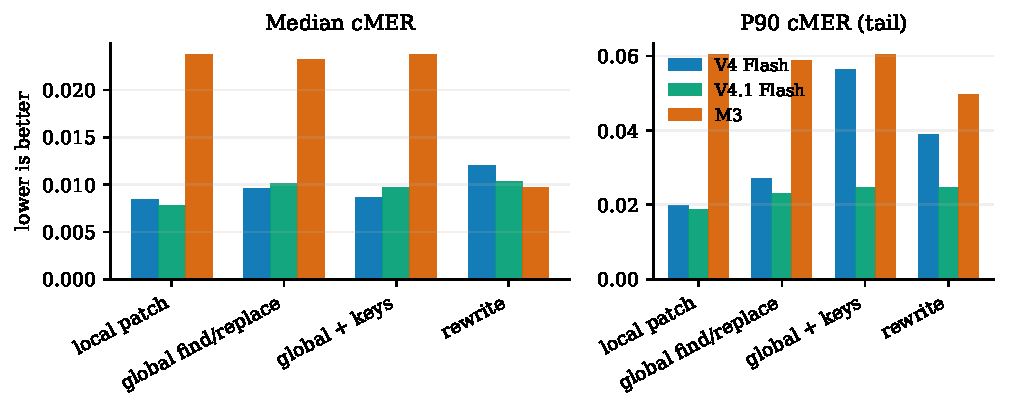
\includegraphics[width=\linewidth]{figures/interface-distributions.pdf}
\caption{Median and P90 per-document cMER for representative interfaces. The local patch condition separates the tail for the two DeepSeek configurations. MiniMax M3 tool arms mostly do not edit, so their values collapse toward the no-edit anchor.}
\label{fig:dist}
\end{figure}

\subsection{The presentation confound}
In the V4 run, changing \fr{} to \textsc{Global+Keys} leaves the replacement tool unchanged and adds numeric keys to the view. Correction rate falls from 61.3\% to 51.0\%, a difference of $-10.3$ percentage points. The cluster-bootstrap 95\% interval is $[-21.1,-1.7]$ percentage points. Edit spans fall from 254.5 to 218.2 (14.2\%), but its cluster interval $[-94.1,8.2]$ includes zero. The safe conclusion is therefore that presentation changed correction behavior in this condition; the edit-span effect is descriptive.

The same comparison on V4.1 is small and uncertain: correction rate changes by approximately $-0.9$ percentage points and the interval crosses zero. This model interaction is why we do not describe numeric keys as a generally harmful presentation choice.

\subsection{Protocol compliance is a first-class outcome}
MiniMax M3 makes the protocol boundary visible. The six tool arms complete between 1 and 15 of 33 tasks; their median cMER is at or near the no-edit anchor, and most cells have zero effective edit spans. By contrast, both rewrite arms complete all 33 tasks. Figure~\ref{fig:m3} plots completion and effective-edit rates. The four tasks that finish in the blocked arm do not contain effective edits despite one low cMER value, so that value must not be interpreted as a successful tool correction.

M3 also exposes key leakage: the rewrite-with-keys arm leaks numeric prefixes in 10 of 33 documents, whereas the rewrite arm without keys and all tool arms do not. This is a model-view interaction, not evidence that stable keys improve rewriting.

\begin{figure}[t]
\centering
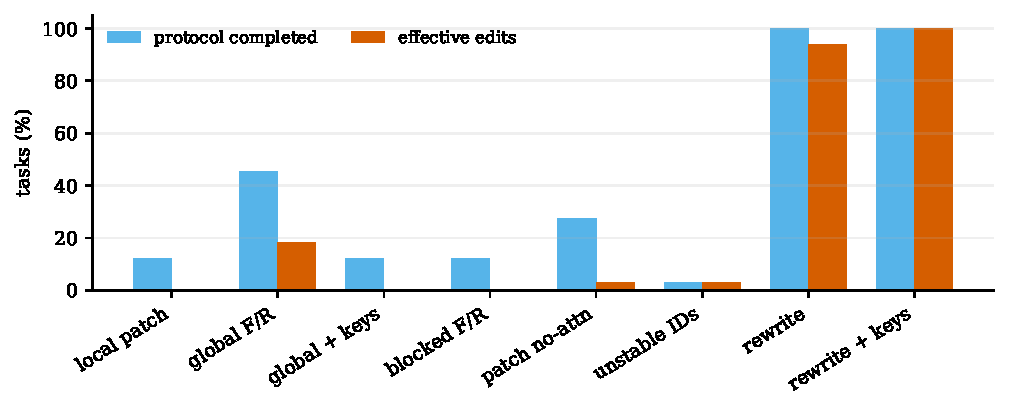
\includegraphics[width=\linewidth]{figures/m3-compliance.pdf}
\caption{MiniMax M3: protocol completion and effective editing. Tool-arm completion is low under the one-shot text grammar, making arm ranking uninterpretable without compliance reporting.}
\label{fig:m3}
\end{figure}

\begin{table}[t]
\centering\small
\caption{Principal results. Values are per-document median / P90 / maximum cMER.}
\label{tab:main}
\begin{tabular}{lccc}
\toprule
Model & Local patch & Global F/R & Rewrite\\
\midrule
DeepSeek V4 Flash & 0.0084 / 0.0199 / 0.0295 & 0.0096 / 0.0272 / 0.0605 & 0.0121 / 0.0389 / 0.9648\\
DeepSeek V4.1 Flash & 0.0078 / 0.0187 / 0.0284 & 0.0101 / 0.0230 / 0.0582 & 0.0104 / 0.0245 / 0.0605\\
MiniMax M3 & 0.0238 / 0.0605 / 0.0659 & 0.0232 / 0.0587 / 0.0621 & 0.0097 / 0.0496 / 0.7342\\
\bottomrule
\end{tabular}
\end{table}

\section{Discussion}
\paragraph{What the results establish.} The strongest empirical result is a distributional one. In two DeepSeek configurations, local, block-scoped editing keeps the worst observed cMER close to 0.03, while global rewriting can produce isolated catastrophic corruption. The median gap is much smaller. This is a useful reliability pattern for OCR systems whose users care about preserving already-correct text.

\paragraph{What the results do not establish.} The study does not establish a universal ranking of editing interfaces, a mechanism-level claim about attention, or a model-independent benefit of stable identifiers. M3 shows that an interface can fail before semantic editing begins. In that regime, treating the no-op-like score as evidence about edit quality would be a category error.

\paragraph{Why the IR matters.} The IR and tape make the interface experiment inspectable. A reviewer can replay a tool fold, distinguish a rejected operation from a model decision to stop, and verify that a failed batch did not partially mutate the document. This is an experimental control benefit in addition to a systems-design benefit.

\section{Limitations and Reproducibility}
The evaluation uses 33 document tasks from one German subset and three matched noise levels. The documents are grouped by source, so the effective independent-document count is 11. Results are one-shot and prompt-sensitive. Two DeepSeek runs share an endpoint family; the M3 run changes protocol and endpoint, so it is not a clean model-only replication. We do not evaluate multilingual data, image-conditioned correction, multi-turn human review, or masked test data.

The document-level scorer in this repository reports per-document cMER and distributional summaries; it is not the official micro-averaged leaderboard score. We release the exact configuration names, prompts, session tapes, IR snapshots, deterministic replay path, and figure-generation script with this manuscript. Before submission, the author metadata and repository URL should be filled in, and the corrected report wording should replace the two historical misinterpretations noted in the accompanying audit.

\section{Conclusion}
A language-model agent does not edit a document in the abstract: it edits through an interface. On HIPE-OCRepair-style OCR correction, a block-addressable interface can reduce rare destructive failures for protocol-compliant DeepSeek configurations, while leaving central performance relatively close to global alternatives. The same study shows why this claim needs guardrails. Presentation alone can change behavior, unstable or full-document views can expose catastrophic tails, and a model that cannot follow the tool grammar cannot be fairly ranked by edit quality. Auditable IR state, replayable tapes, tail-aware metrics, and explicit compliance rates should be treated as part of the evaluation protocol.

\bibliographystyle{unsrtnat}
\bibliography{references}

\appendix
\section{Interface prompts and audit details}
The stable-key view labels each block with an immutable integer identifier and states that identifiers are not line numbers. The local tool accepts \texttt{read(path)}, \texttt{find\_replace(path,key,old,new)}, and \texttt{done()}; uniqueness is checked within the selected block. The global tool accepts the same grammar without a key and checks uniqueness over the complete document. The attention condition adds a two-pass instruction: inspect each block independently, then use cross-block evidence before emitting calls. The no-attention control removes this instruction while leaving the view and tool implementation unchanged.

The report's fixed rate measures corrected input errors, while broken rate measures newly introduced errors relative to already-correct input characters. Key leakage is reported separately from correction quality. A cell with no effective edits can still have low cMER if its input is easy; therefore we report edit spans and the no-edit anchor alongside cMER.

\end{document}
